\chapter{Notions of infrared thermography}

	\section{Infrared radiation spectrum.}
	
		Infrared (IR) radiation is the energy irradiated by a surface that has a temperature above the absolute zero [1]. Within the electromagnetic spectrum, IR radiation is defined as the radiation band that spans from 0.7 $\mu$m to 1000 $\mu$m in wavelength (Figure \ref{fig1}).\\ Much of the IR spectrum, however, is not useful for Infrared thermography (IRT) due to atmospheric absorption. This absorption occurs mainly with $H_{2}O$ and $CO_{2}$ molecules as they are well known for being good heat absorbers (Figure \ref{fig2}). According to this fact, the IR wavelength range is sometimes further divided into 4 additional categories:

		\begin{enumerate}[I.]
			\item Near-infrared (NIR) from 0.8 $\mu$m to 1.7 $\mu$m.
			\item Short-wavelength infrared (SWIR) from 1 $\mu$m to 2.5 $\mu$m.
			\item Mid-wavelength infrared (MWIR) from 2 $\mu$mm to 5 $\mu$mm.
			\item Long-wavelength infrared (LWIR) from 8 $\mu$mm to 14 $\mu$mm.
		\end{enumerate}
		
		\begin{figure}[ht!]
			\centering
			\captionsetup{justification=centering,margin=2cm}
			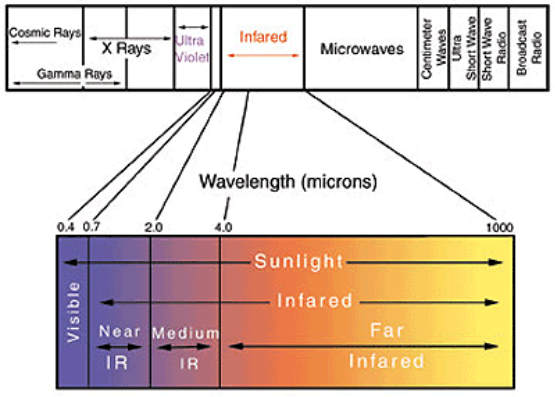
\includegraphics[scale=0.75]{Figures/Chapter01/lightspectrum}
			\caption{\label{fig1} Electromagnetic spectrum showing the portion corresponding to IR radiation.}
		\end{figure}
		
		It is important to note that this classification is somewhat arbitrary and therefore it can change quite a bit from one author to the other but in general they remain fairly similar. Most IR sensors are designed to work in the LWIR part of the spectrum since this is the range that minimizes this absorptions.\\ In this study, as we use an IR camera sensitive only to the fourth type, we will refer to IR as the LWIR except otherwise explicitly stated.
		
		\begin{figure}[ht!]
			\centering
			\captionsetup{justification=centering,margin=2cm}
			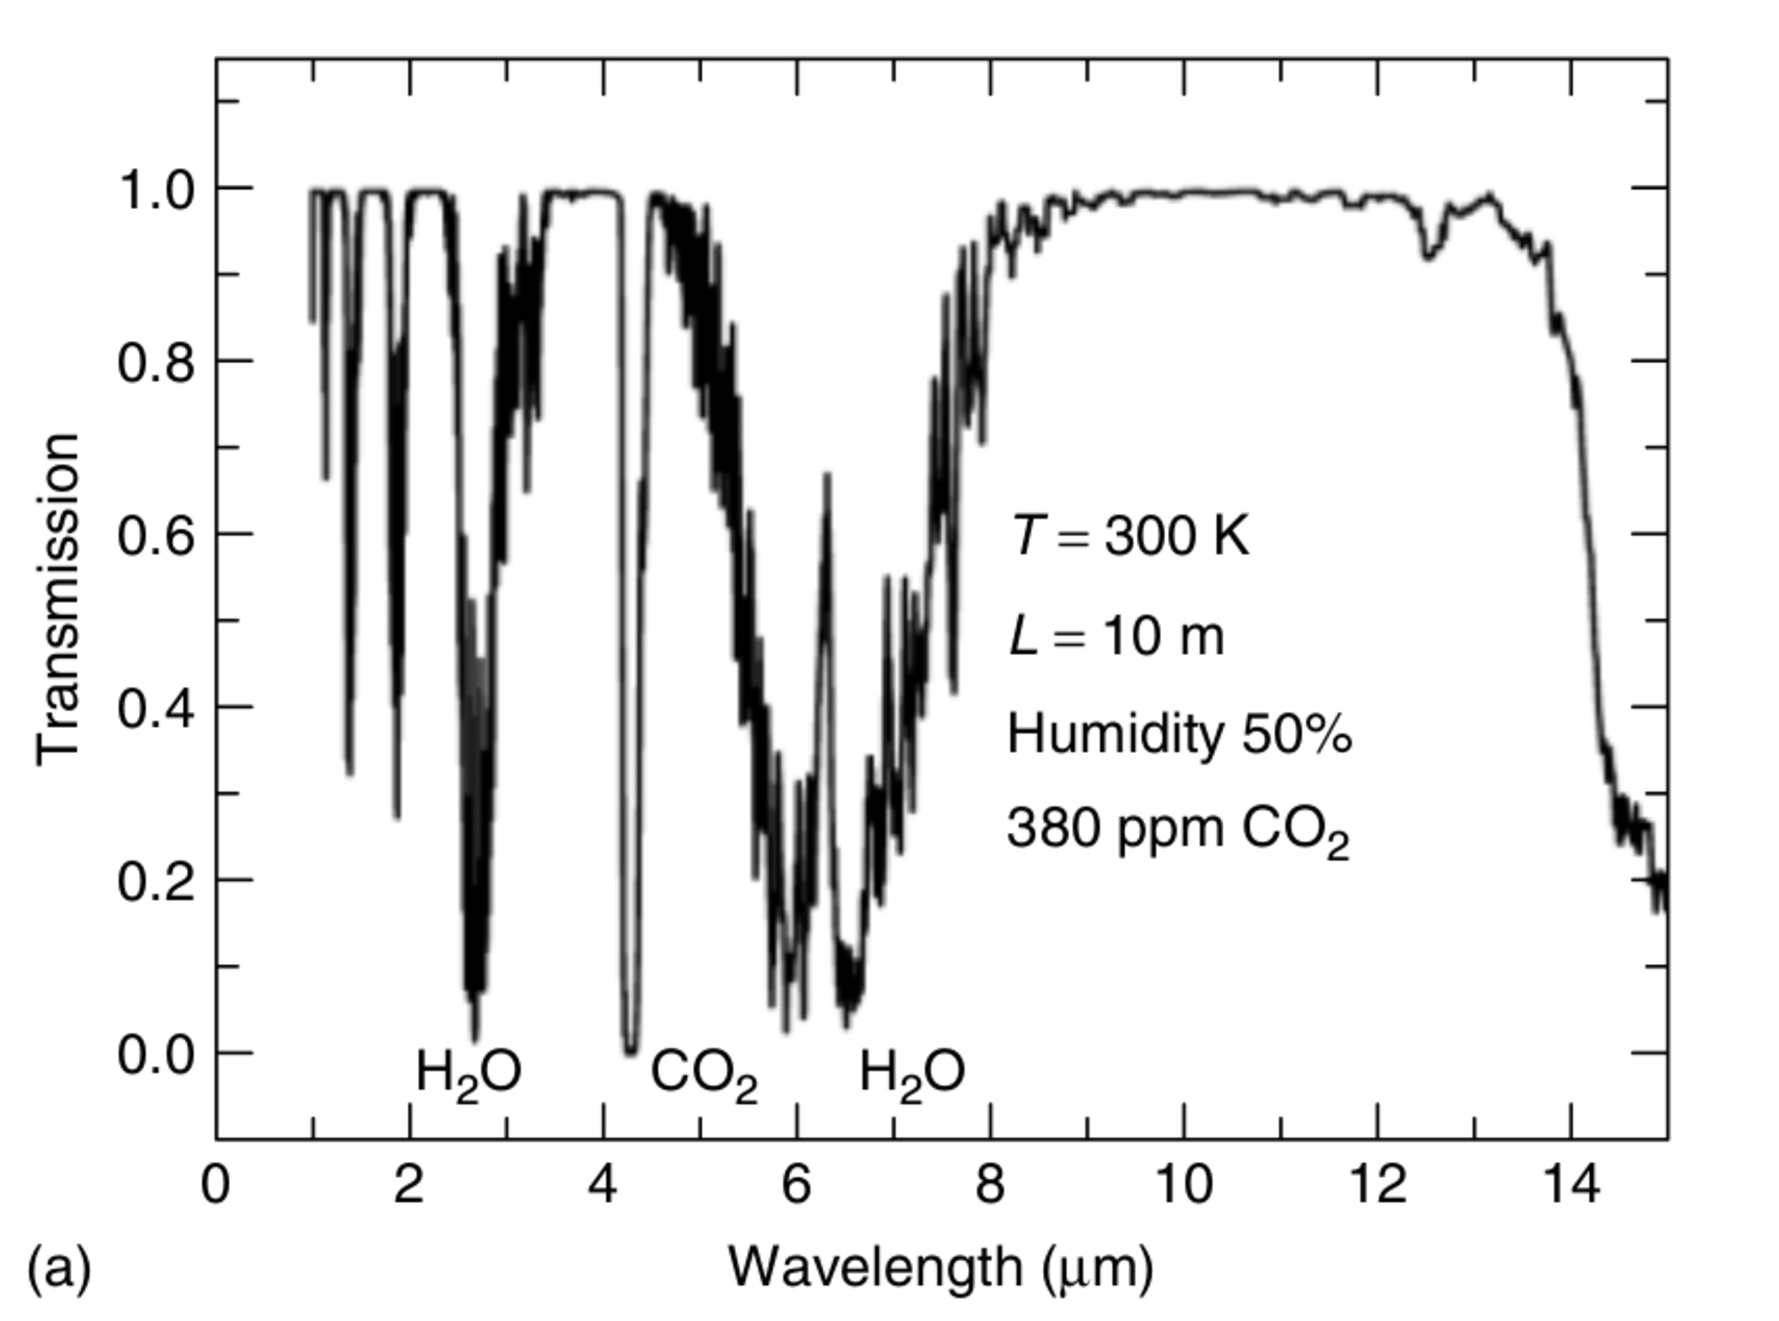
\includegraphics[scale=0.45]{Figures/Chapter01/Transmission.pdf}
			\caption{\label{fig2} A typical atmospheric transmittance plot  for infrared radiation. For some of the minima we can see the absorbing molecule responsible,}
		\end{figure}
		
	\section{Plank's law for blackbodies. IR radiation dissipation.}
	
		According to Plank's law, the IR emissive power of a blackbody at a temperature $T$, with a wavelength between $\lambda$ and $\lambda+d\lambda$ is given by equation (\ref{eq1}), where $C_{1}$ and $C_{2}$ are constants, often called first and second radiation constants respectively [2].
		
		\begin{equation}
			\label{eq1}
			N_{b}(\lambda,T)d\lambda=\frac{C_{1} \cdot \lambda^{-5}}{\exp (\frac{C_{2}}{\lambda\cdot T}) -1} d\lambda
		\end{equation}
		
		Figure \ref{fig3} shows this functional dependence for six different temperatures [3]. The gray line represents the displacement of the maximum for each temperature. Note that, as the temperature decreases, the maximum emissive power moves to higher wavelengths, this is known as the Wien's displacement law [4]. 
		
		There are three ways by which the emissive power striking an object may be dissipated: absorption, transmission and reflection [5]. The fractions of the total radiant energy that are associated with each of these modes of dissipation are referred to as the \textit{absorptivity}, \textit{transmissivity} and \textit{reflectivity} of the body. Three parameters are used to describe these phenomena: the spectral \textit{absorptance} $\alpha$, which is the fraction of the spectral emissive power absorbed by the object, the spectral \textit{reflectance} $\rho$, which is the fraction of the spectral emissive power reflected by the object, and the spectral \textit{transmittance} $\tau$, which is the fraction of the spectral emissive power transmitted by the object.
		
		\begin{figure}[ht!]
			\centering
			\captionsetup{justification=centering,margin=2cm}
			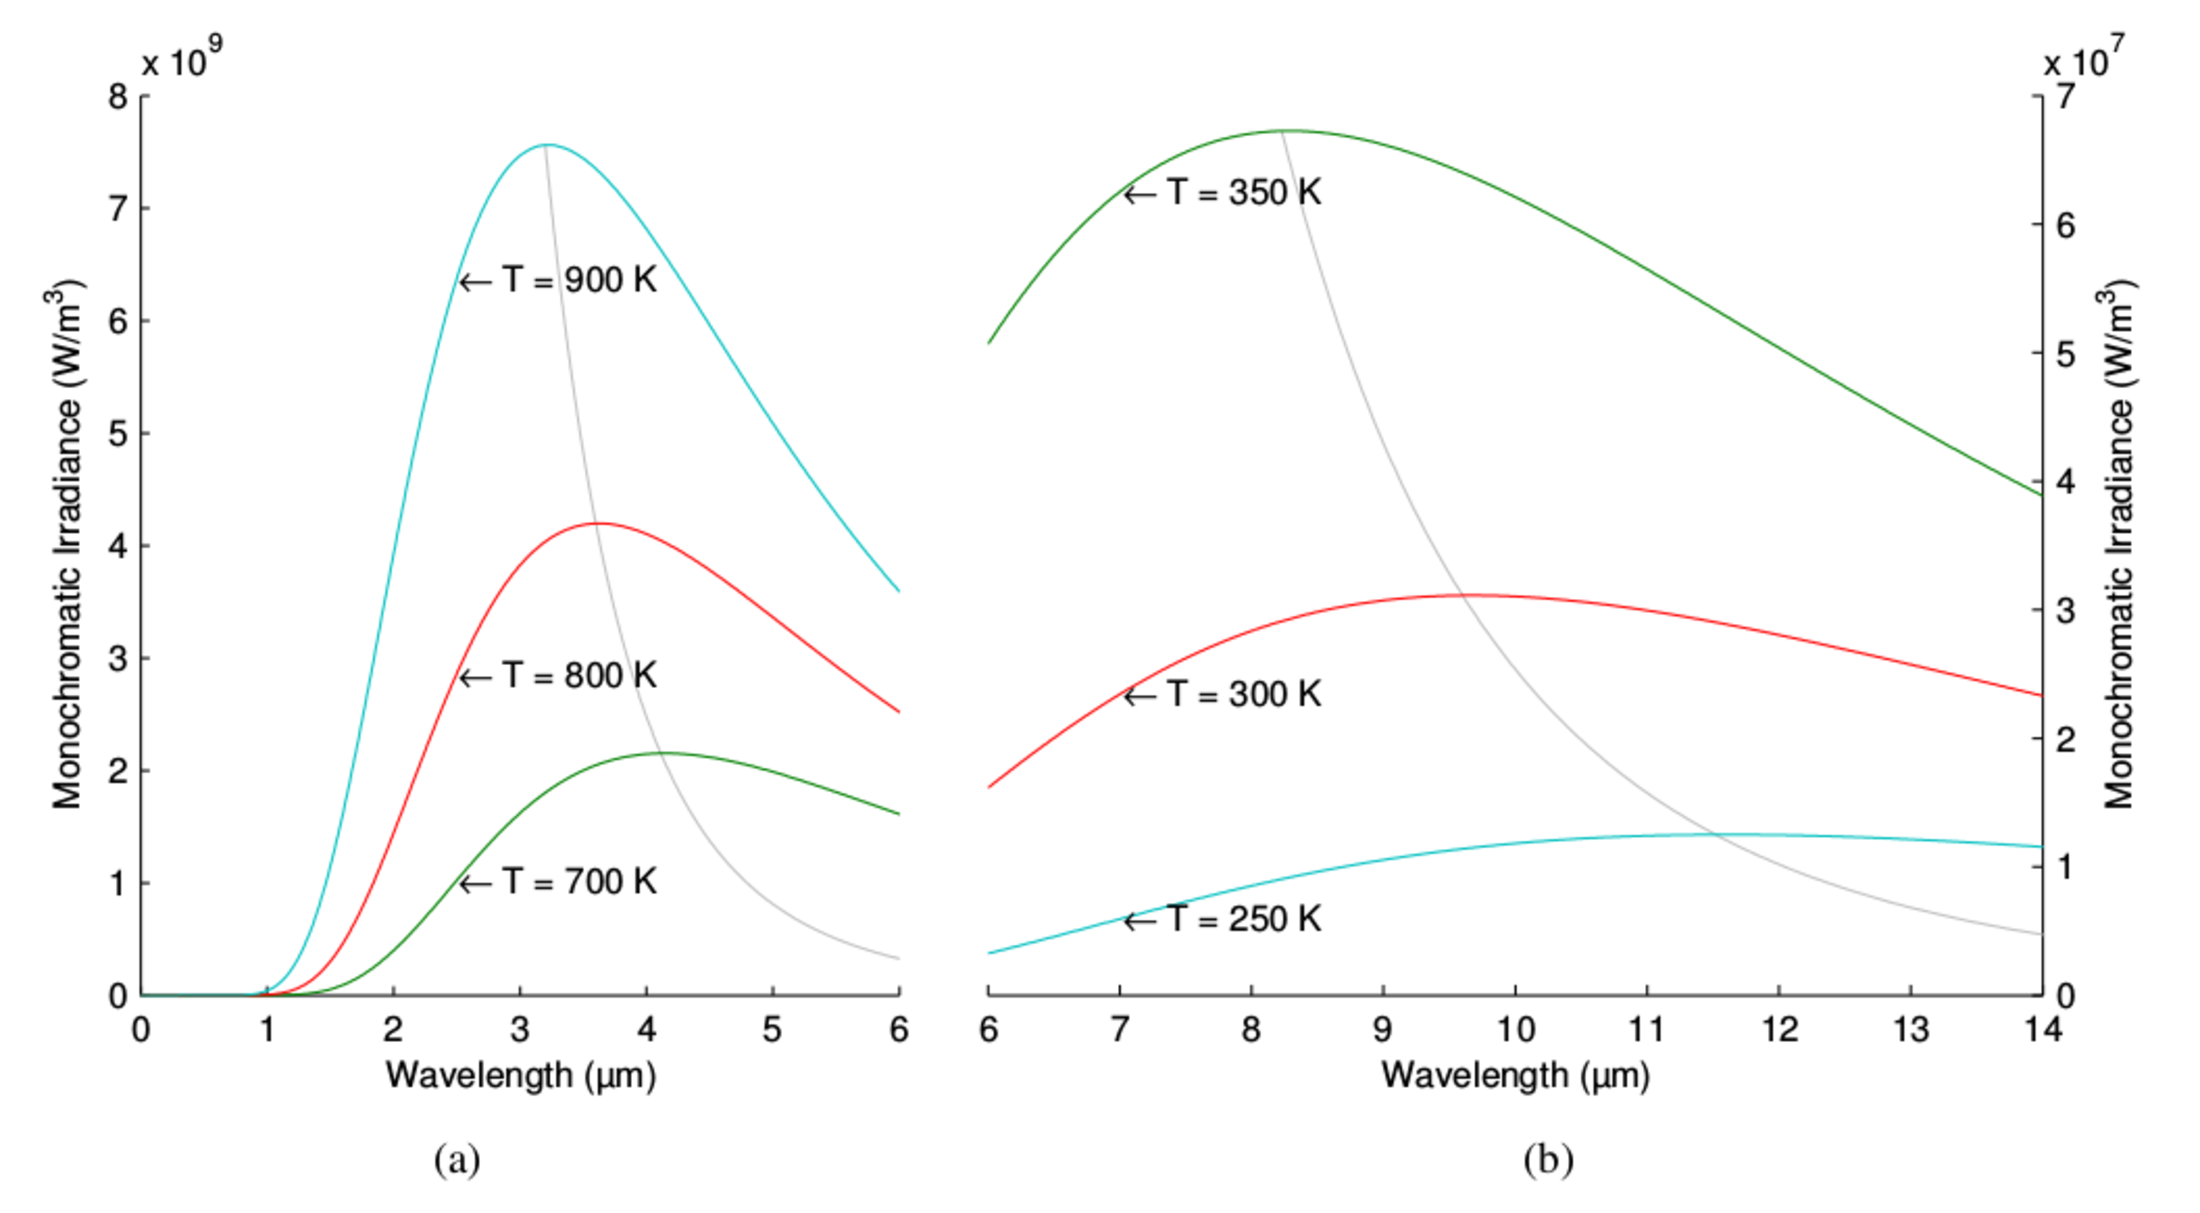
\includegraphics[scale=0.45]{Figures/Chapter01/PlankFunction.pdf}
			\caption{\label{fig3} Planck's law: electromagnetic radiation emitted by a blackbody in thermal equilibrium at a definite  temperature. (a) Objects with a high temperature emit most of the radiation in the middle wave infrared; (b) Objects with a low temperature emit most of the radiation in the long wave infrared. The two parts of the graph are scaled differently on the y-axis.}
		\end{figure}		
		
		These three parameters are, in general, wavelength dependent and their sum must be one at any given wavelength and surface temperature:
		
		\begin{equation}
			\label{eq2}
			\alpha + \rho + \tau = 1
		\end{equation}	
		
			